%Binaural Reproduction of Plane Waves With
%Reduced Modal Order
%
%Binaural rendering of Ambisonic signals by head-related impulse response time
%alignment and a diffuseness constraint
%
%HRTF——Note
%
%Insights into head-related transfer function: Spatial
%dimensionality and continuous representation
%
%可以参考: Interaural cross correlation in a sound field represented by spherical harmonics
%里面包括了双耳信号获取和HRTF分量求解。 已下载,已打印,other标号。

\chapter{基于~HRTF~球谐分解的双耳渲染算法} \label{chapter.HRTF}

对~HRTF~进行球谐分解并在球谐域上直接渲染的双耳渲染算法近年来得到了广泛关注,本章将在~\ref{sec.SHdecomposition}~节的基础上对其进行详细介绍,其包含两个同等重要的部分:声场和~HRTF。在声场获取方面,麦克风阵列尤其是球形麦克风阵列可以更好地采集声场的特征,具有高质量、高保真的录制效果,是多通道录制与重构、空间音频技术的重要工具。首先对空心球和刚性球进行讨论和对比,分别给出其球谐系数的求解方法。接下来对~HRTF~的获取和其球谐分量的求解方法进行介绍。并且在此基础上,对~HRTF~的预处理方法的原理进行详细介绍,该方法可以有效降低~HRTF~的球谐分解阶次。最后通过实验验证了预处理方法的有效性。

\section{球形麦克风阵列的声场录制及球谐系数估计}\label{section_microphone_array_coe}
声场录制的关键在于如何准确获得待录制声场的高阶球谐系数,使用球形麦克风阵列可以实现此目标。球形麦克风阵列是通过将麦克风放置在三维空间中并记录麦克风所在位置的声压信号来实现的。影响球阵可以准确重现声场的因素包括频率、阵列半径、阵元数目和球面采样方式等~\tcite{SMA_design}。
录制声场球谐系数的估计依赖于麦克风阵列的采样配置,在一些特殊的采样方式~\tcite{rafaely_fundamentals_2019}~例如等角采样、高斯采样和均匀采样(如图~\ref{fig:sampling}~所示)的情况下,可以使用求和来代替积分计算录制声压的球谐系数,能够方便地计算函数的球傅里叶变换。在实际系统中很难要求所有球阵满足特殊的采样方式,因此需要给出在任意采样配置下使用球傅里叶变换来计算球谐系数的方法。

\begin{figure}[!h]
\centering
\includegraphics[width=0.85\textwidth]{figure/chapter3/sampling-eps.pdf}
\caption{ 球面采样:(a)~等角采样;
(b)~高斯采样;(c)~均匀采样。}\label{fig:sampling}
\end{figure}

%%%%%%%%%%%%%%%%%%%%% 开球和刚性球 %%%%%%%%%%%%
使用半径为~$R$~的球形麦克风阵列采集来自~$(\theta_s,\phi_s)$~的单位幅度平面波时,麦克风~$(\theta _q,\phi _q)$~ 连续分布在球面上。此处假设声源均位于球形麦克风阵列外,麦克风观测声压可分为空心球和刚性球两种情况进行讨论~\tcite{williams_fourier_2000,rafaely_fundamentals_2019}。

\subsection{空心球的球谐系数估计}

对于空心球来说,忽略单个麦克风和支架对声波的影响,可以认为其录制的声场即为真实环境下的声场,直接进行球谐系数的估计。

对于特殊的采样方式,球面积分可以通过~$Q$~个球面采样~$(\theta_{q},\phi_{q})$~的加权求和来逼近,如式~\eqref{eq.sum_integral}~所示:
\begin{equation}\label{eq.sum_integral}
   \int_{0}^{2\pi}\int _{0}^{\pi} g(\theta,\phi) \sin\theta d\theta d\phi \approx \sum_{q=1}^{Q} \alpha_{q} g(\theta_{q},\phi_{q}),
\end{equation}
其中,$\alpha_{q}$~是采样权重,式~\eqref{eq.Equal_angle_sampling}、\eqref{eq.Gaussian_sampling}~和~\eqref{eq.uniform_sampling}~分别为等角采样、高斯采样和均匀采样下的权重表达式:
\begin{equation}\label{eq.Equal_angle_sampling}
\alpha_{q}=\frac{2 \pi}{(N+1)^{2}} \sin \left(\theta_{q}\right) \sum_{q^{\prime}=0}^{N} \frac{1}{2 q^{\prime}+1} \sin \left(\left[2 q^{\prime}+1\right] \theta_{q}\right).
\end{equation}
\begin{equation}\label{eq.Gaussian_sampling}
\alpha_{q}=\frac{\pi}{N+1} \frac{2\left(1-\cos ^{2} \theta_{q}\right)}{(N+2)^{2}\left[P_{N+2}\left(\cos \theta_{q}\right)\right]^{2}}.
\end{equation}

\begin{equation}\label{eq.uniform_sampling}
   \alpha_{q} = \frac{4\pi}{Q}.
\end{equation}

则通过球傅里叶变换获取球谐系数的式~\eqref{eq.SFT}~可以表示为:
\begin{equation}\label{eq.sample_coe}
   S_n ^m(r,f)=\sum_{q=1}^{Q} \alpha_{q} S(r,\theta_{q},\phi_{q},f)[{Y_n^{m}(\theta_{q},\phi_{q})}]^{*}.
\end{equation}
此时,球谐系数可以直接采用上式进行求解。

在某些情况下,从这些或其他预定义的采样配置中选择采样集可能是不可行的,例如,由于麦克风定位的机械限制。因此,在任意给定采样集时,如何计算球面球谐系数在实际应用中具有重要的价值。考虑在单位球面上进行采样,根据球傅里叶变换,第~$q$~个麦克风的接收信号可以写为:
\begin{equation}\label{eq.coe_random_sampling}
   S(r,\theta_{q},\phi_{q},f)=\sum _{n=0}^{N_{s}}\sum _{m=-n}^n S_n ^m(r,f)Y_n ^m(\theta,\phi),
\end{equation}
其矩阵形式为:
\begin{equation}\label{eq.coeMat_random_sampling}
\bm{S}=\bm{Y S_{nm}},
\end{equation}
其中,$\bm{S}$~和~$\bm{S_{nm}}$~是长度为~$Q$~和~$(N_{s}+1)^2$~的列向量,$\bm{Y}$~是大小为~$Q\times(N_{s}+1)^2$~的矩阵,
\begin{equation}
\bm{S} = [S(r,\theta_{1},\phi_{1},f),~S(r,\theta_{2},\phi_{2},f)~,~\cdots~,~S(r,\theta_{Q},\phi_{Q},f)]^{T},
\end{equation}
\begin{equation}
\bm{S_{nm}} = [S_{0}^{0}~,\cdots,~S_{n}^{m}~,~\cdots~,~S_{N_{s}}^{N_{s}}]^{T},
\end{equation}

\begin{equation}
\bm{Y}=\left[
\begin{array}{ccccc}
Y_{0}^{0}\left(\theta_{1}, \phi_{1}\right) & \cdots & Y_{n}^{m}\left(\theta_{1}, \phi_{1}\right) & \cdots & Y_{N_{s}}^{N_{s}}\left(\theta_{1}, \phi_{1}\right) \\
Y_{0}^{0}\left(\theta_{2}, \phi_{2}\right) & \cdots &  Y_{n}^{m}\left(\theta_{2}, \phi_{2}\right) & \cdots & Y_{N_{s}}^{N_{s}}\left(\theta_{2}, \phi_{2}\right) \\
\vdots  & \ddots & \vdots  & \ddots & \vdots \\
Y_{0}^{0}\left(\theta_{Q}, \phi_{Q}\right) & \cdots & Y_{n}^{m}\left(\theta_{Q}, \phi_{Q}\right) & \cdots & Y_{N_{s}}^{N_{s}}\left(\theta_{Q}, \phi_{Q}\right)
\end{array}\right].
\end{equation}

当~$Q=(N+1)^2$~时,式~\eqref{eq.coeMat_random_sampling}~的解可以通过矩阵~$\bm{Y}$~的逆求解(要求球形麦克风阵列的采样位置满足矩阵~$\bm{Y}$~可逆的条件):
\begin{equation}
\bm{S_{nm}} = \bm{Y}^{-1}\bm{S},
\end{equation}
在许多情况下都使用过采样,即~$Q>(N+1)^2$,此时式~\eqref{eq.coeMat_random_sampling}~超定,其最小二乘解由矩阵的伪逆给出::
\begin{equation}
\bm{S_{nm}} = \bm{Y^{\dagger}} \bm{S}= (\bm{Y}^{H}\bm{Y})^{-1}\bm{Y}^{H}\bm{S}.
\end{equation}
当~$Q<(N+1)^2$~时,采样点数不足,式~\eqref{eq.coeMat_random_sampling}~可能不能提供正确的解。

\subsection{刚性球的球谐系数估计}

和空心球相比,刚性球录制的总声压场,也就是实验中的被测声压,可以分为入射声场和散射声场两个部分。从实验的角度来说,入射声场是针对球体不存在时测量的声压场,而散射声场是球体存在时声压场的变化量。对于刚性球来说,其表面的径向速度为~0,即球体表面处入射场和散射场的总径向速度为~0,满足~Neumann~边界条件~\tcite{williams_fourier_2000}。如果散射场为零,则认为该球体是完全可透射的。
% 对于释压球来说,其在球体表面上的总声压为~0。

大多数散射问题的研究都是从平面波着手的,对于来波方向为~$(\theta_s,\phi_s)$~的单幅度平面波来说,麦克风~$(r,\theta _q,\phi _q)$~处观测到的入射声压(直达声)可以用球贝塞尔函数表示:
\begin{equation}  \label{SMic_pressure open}
   S_{\mathrm{dir}}(r,\theta _q,\phi _q,f)=\sum _{n=0}^{\infty}4\pi i^n j_n(kr)\sum _{m=-n}^{n}[Y_n ^{m}(\theta_s,\phi_s)]^*Y_n ^{m}(\theta_q,\phi_q).
\end{equation}
上式即为空心球情况下麦克风的接收信号。

因为散射声场代表了入射声波在球面的散射而发出的球面声波,因此散射声压可以利用表示去波的第一类球汉克尔函数展开:
\begin{equation}  \label{SMic_pressure scat}
   S_{\mathrm{scat}}(r,\theta _q,\phi _q,f)=-\sum _{n=0}^{\infty}4\pi i^n \frac{j'_n (kr)}{({h^{(1)}_n})'(kr)}h_n^{(1)}(kr)\sum _{m=-n}^{n}[Y_n ^{m}(\theta_s,\phi_s)]^*Y_n ^{m}(\theta _q,\phi _q),
\end{equation}
其中,$j_n'(kr)$~和~$({h^{(1)}_n})'(kr)$~分别为~$n$~阶球贝塞尔函数~$j_n(kr)$~和~$n$~阶第一类球汉克尔函数~$h_n^{(1)}(kr)$~的导数。波动方程在频域上的表示称为亥姆霍兹方程,球坐标系下亥姆霍兹方程中只与距离相关的项所构成的方程被称为球贝塞尔方程,球贝塞尔函数和球汉克尔函数共同组成了球贝塞尔方程的解。

对于刚性球来说,麦克风的录制信号中除了直达声外,还包含因球面散射形成的散射声,则接收到的总声压可表示为:
\begin{align}  \label{SMic_pressure rigid}
   S(r,\theta_q,\phi_q,f)&= S_{\mathrm{dir}}(r,\theta_q,\phi_q,f)+S_{\mathrm{scat}}(r,\theta_q,\phi_q,f)   \nonumber \\
   &=\sum _{n=0}^{\infty} 4\pi i^n \left( j_n(kr)-\frac{j'_n (kr)}{({h^{(1)}_n})'(kr)}h_n^{(1)}(kr) \right) \sum _{m=-n}^{n}[Y_n ^{m}(\theta_s,\phi_s)]^*Y_n ^{m}(\theta_q,\phi_q),
\end{align}

整合公式~\eqref{SMic_pressure open}~和式~\eqref{SMic_pressure rigid},可以得到采用不同麦克风阵列时,第~$q$~个麦克风接收信号的表达式:
\begin{equation}  \label{SMic_pressure}
   S(r,\theta_q,\phi_q,f)=
   \sum _{n=0}^{\infty} b_n(kr) \sum _{m=-n}^{n}[Y_n ^{m}(\theta_s,\phi_s)]^*Y_n ^{m}(\theta_q,\phi_q),
\end{equation}
其中,$b_n$~表示模态强度:
\begin{equation}\label{eq.bn(kr)}
b_n(kr) =
\begin{cases}
 4\pi i^n j_n(kr)  & ~\mbox{空心球} \\
 4\pi i^n \left(j_n(kr)-\frac{j'_n (kr)}{({h^{(1)}_n})'(kr)}h_n^{(1)}(kr) \right) & ~\mbox{刚性球}.
\end{cases}
\end{equation}


\begin{figure}[H]
\centering
\subfigure[]{
\includegraphics[width=0.48\textwidth]{figure/chapter3/bn_open}}
\hfill
\subfigure[]{
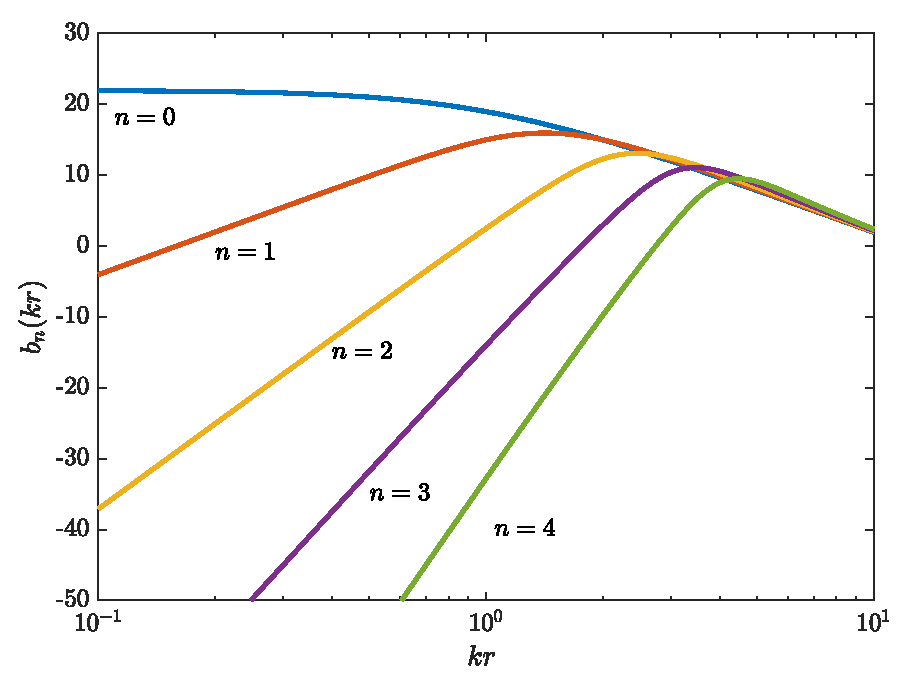
\includegraphics[width=0.48\textwidth]{figure/chapter3/bn_rigid}}
\caption{模态强度~$b_n$:(a)~空心球模态强度; (b)~刚性球模态强度}
\label{fig:bn}
\end{figure}

图~\ref{fig:bn}~为模态强度~$b_n$~随~$kr$~的变化趋势图。(a)~中曲线有很深的凹陷,即在某些频率处模态强度为~0。而~(b)~中刚性球可以避免空心球所带来的凹陷(零点)问题,这是因为刚性球麦克风接收到的不仅包含直达声还有声波入射到球体产生的散射声。关于零点问题带来的影响将在第~\ref{sec.modelAndMusic}~节中关于球谐域~MUSIC~定位算法和第~\ref{subsec.open_rigid}~节中的实验结果进行展现。

并且由于散射声场的存在,在高阶次和低频率的情况下,刚性球模态强度的幅度稍大于空心球,因此刚球对传感器噪声和其他误差的影响的鲁棒性有些许提升~\tcite{rafaely_fundamentals_2019}。另外,实际情况下由于麦克风数目较多,所以做成刚性球更合理,目前常用的刚球为~32~通路~Eigenmike~\tcite{microphone}。

%在求解刚性球录制声场的球谐分量时,在根据式~\eqref{eq.coe_random_sampling}~计算得到~$S_n ^m(r,f)$~之后需要一定的转换,以避免球面散射带来的影响。
%
%\begin{equation}\label{eq.coe_eigen}
%S_{nm}^{rigid}(r,f) = \frac{ S_n^m(r,f) }{j_n(kr)-\frac{j'_n (kr)}{[{h^{(1)}_n}]'(kr)}h_n^{(1)}(kr) } j_n(kr)
%\end{equation}
%
%通过式~\eqref{eq.coe_eigen}~即可求解原始无刚球情况下的球谐分量。

\section{~HRTF~的球谐分解}\label{sec.SHcoe_HRTF}

本节将对头相关传递函数~HRTF~的三种获取方式以及本文所采用的两种数据库加以介绍,并且给出了如何从给定~HRTF~数据库中求解~HRTF~球谐系数的方法。


\subsection{HRTF~的获取}
HRTF~和~HRIR~是双耳渲染算法中合成双耳信号的重要数据基础,其可以通过计算、定制与测量三种方法获取~\tcite{book_xiebosun}。

原则上,声波经由头部、耳廓、躯干等生理结构的综合滤波过程可以通过求解加以边界条件约束的波动方程来获得,即边界元法(boundary element method,BEM)\tcite{katz2001boundary}。但实际上边界表面的不规则性会产生及其复杂的现象,以足够的准确度实现边界表面(尤其是耳廓)的测量具有一定的挑战,并且计算量较大。还有一些分析解决方案适用于非常简单的几何形状,在简化情况下,忽略耳廓和躯干的影响,将头部近似为刚性球体。在此基础上,雪人模型~\tcite{algazi2002approximating}~将头部和躯干简化为两个不同半径的球,并采用多重散射或多级展开的方法进行求解,数学方法非常复杂。目前已知的仿真~HRTF~数据库为~MESH2HRTF~\tcite{HRTF_MESH2HRTF},其采用边界元法,频率范围为~100Hz~到~22kHz,以~100Hz~为间隔,球面采样点数为~4334~个,采样方式为列别捷夫采样。

~HRTF~的定制主要应用于获取个性化~HRTF~,假定~HRTF~和一定的生理参数之间存在高的相关性。主要包括生理参数匹配法、频率标度变换法和生理参数线性回归法,近几年也出现了基于机器学习的个性化~HRTF~生成模型。总体上,定制~HRTF~较测量和计算来说比较简单,且可以得到一定的效果,但其准确性有待进一步改进~\tcite{book_xiebosun}。% (摘自《空间声原理》)

现有的技术中,实验测量是获得~HRTF~最重要且最准确的手段~\tcite{book_xiebosun},一个扬声器在特定的位置产生一个脉冲或其他宽带信号,然后通过记录放置在人工头或真人受试者耳道内的两个麦克风的输出信号来测量。根据~HRTF~的定义,理想情况下的测量应该在自由场(消声室)的环境下进行,但实际中也经常采用非消声室的测量方法,为了避免环境反射声的影响,会加以时间窗处理。

双耳麦克风的尺寸很小可以放置在耳道入口处,并使用泡沫环保持在适当的位置,这被称为封闭耳道法,进入耳道的信号被麦克风捕获并存储为双通道录音。封闭耳道法经常用于~HRTF~的测量~\tcite{book_immersive}。

目前国际上已有许多课题组对人工头和真人受试者的远场~HRTF/HRIR~进行了测量,建立了相应的数据库~\tcite{book_xiebosun},大多数数据库都是在远场条件下进行测量,但也有部分是在近场进行。
现有的较为常用的远场~HRTF~数据库包括~MIT~数据库~\tcite{hrtf_MIT}~和~CIPIC~数据库~\tcite{hrtf_CIPIC},其对应的数据已在网上公开。
% (http://sound.media.mit.edu/resources/KEMAR.html~和~http://www.ece.ucdavis.edu/cipic/spatial-sound/hrtf-data)。

除此之外,Benjamin~Bernschutz~使用~Neumann~KU-100~建立了一个远场~HRTF~数据库~\tcite{Benjamin2013A},测量环境为消声室,共采用了~4~种球面采样方式,包括在以~$1^{\circ}$~为角度间隔的圆周上均匀采样,2354、2702~点球面列别捷夫采样和以~$2^{\circ}$~为间隔的球面高斯采样(共计~16020~个采样点),此数据库将在第~\ref{sec.Pre_result}~节用于体现~HRTF~预处理的结果展示。


本文主要采用~CIPIC~数据库进行双耳渲染,其来自加州大学戴维斯分校~CIPIC~交互实验室。在非消声室环境下,对~43~名真人受试者(27~男,16~女)进行测量,是目前真人~HRTF~数据库中空间分辨率较高,同时受试者人数较多的一个,同时给出了真人受试者的生理尺寸~\tcite{book_xiebosun}。
其测量环境为非消声室环境,测量方法为封闭耳道法,~HRIR~的长度为~200~点,采样频率为~44.1~kHz。其测量时采用双耳极坐标系统,如图~\ref{fig:CIPIC_location}~(a)~所示,其中,$(\varTheta,\varPhi) = (0^{\circ},0^{\circ})$~为正前方,$(\varTheta,\varPhi) = (90^{\circ},0^{\circ})$~为正右方。

\begin{figure}[H]
\centering
\subfigure[]{
\includegraphics[width=0.3\textwidth]{figure/chapter3/binaural_cor}}
\hfill
\subfigure[]{
\includegraphics[width=0.6\textwidth]{figure/chapter3/cipic}}
\caption{CIPIC~数据库角度说明:(a)~双耳极坐标系~\tcite{book_xiebosun},(b)~声源位置分布}
\label{fig:CIPIC_location}
\end{figure}

如图~\ref{fig:CIPIC_location}~(b)~所示,CIPIC~数据库共包括~1250~个测量位置,50~个俯仰角为~$\varTheta = -45^{\circ}+5.625^{\circ}\times (0:1:49)$,每个俯仰角均对应~25~个方位角,且非均匀分布,其设定为:
\begin{equation*}
\left[-80~-65~-55~-45:~5:~45~~55~~65~~80\right]
\end{equation*}


以~003~号受试者为例,当声源位于水平面且方位角为~$80^{\circ}$~时,即声源位于右耳方向附近,左右耳的~ITD~和~ILD~取接近最大值,对应的左、右耳的~HRIR~和~HRTF~如图~\ref{fig:CIPIC_80du}~所示。
方位角为~$0^{\circ}$~时,即声源位于正前方,如图~\ref{fig:CIPIC_80du}~所示。

\begin{figure}[H]
\centering
\subfigure[]{
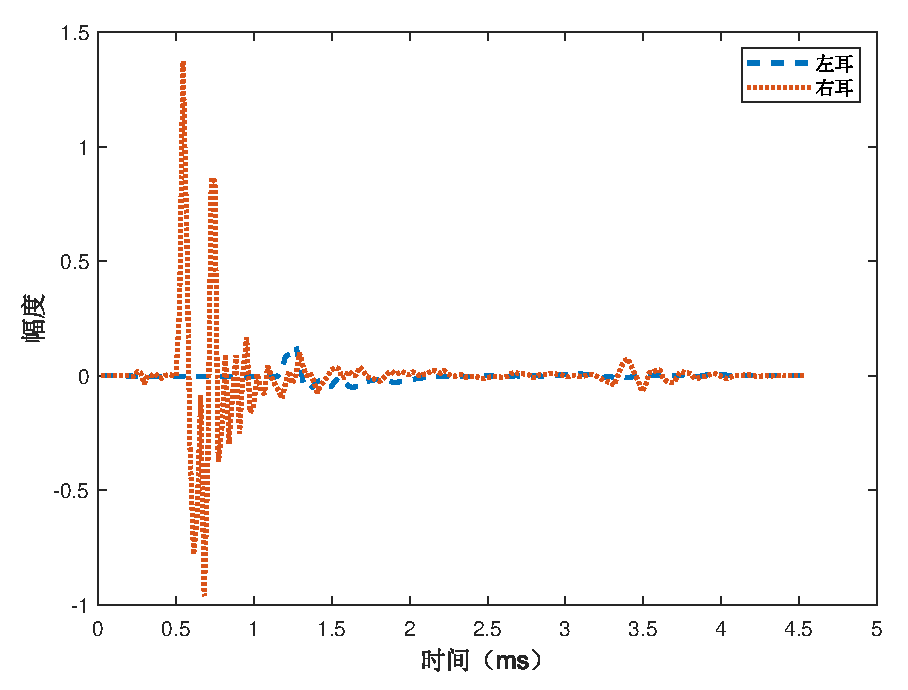
\includegraphics[width=0.48\textwidth]{figure/chapter3/80du_HRIR}}
\hfill
\subfigure[]{
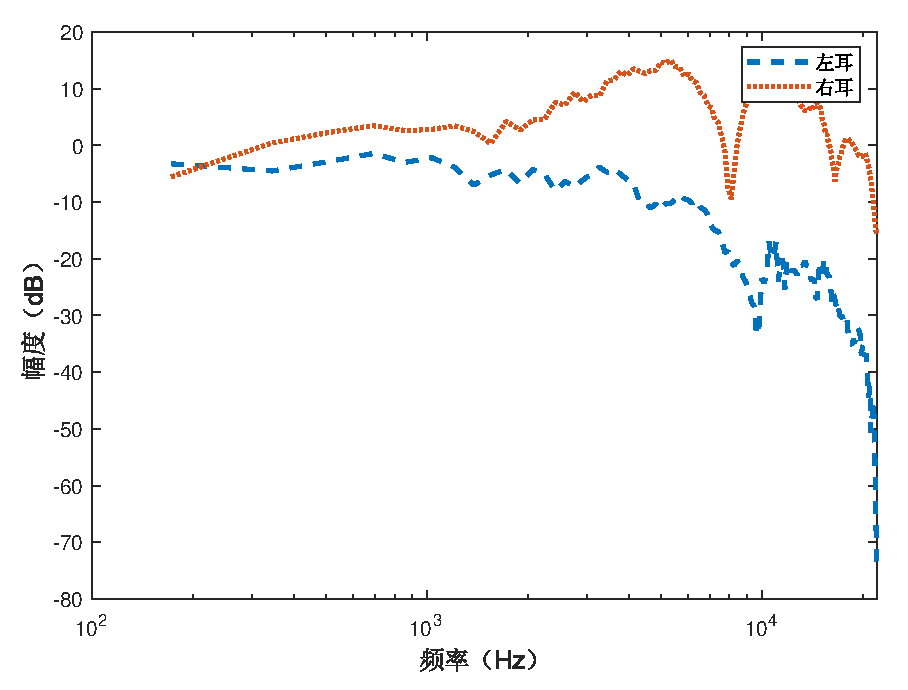
\includegraphics[width=0.48\textwidth]{figure/chapter3/80du_HRTF}}
\caption{CIPIC~数据库中声源位于水平面且方向为~$80^{\circ}$~时的左右耳~HRIR~和~HRTF~数据:(a)~HRIR,(b)~HRTF}
\label{fig:CIPIC_80du}
\end{figure}

\begin{figure}[H]
\centering
\subfigure[]{
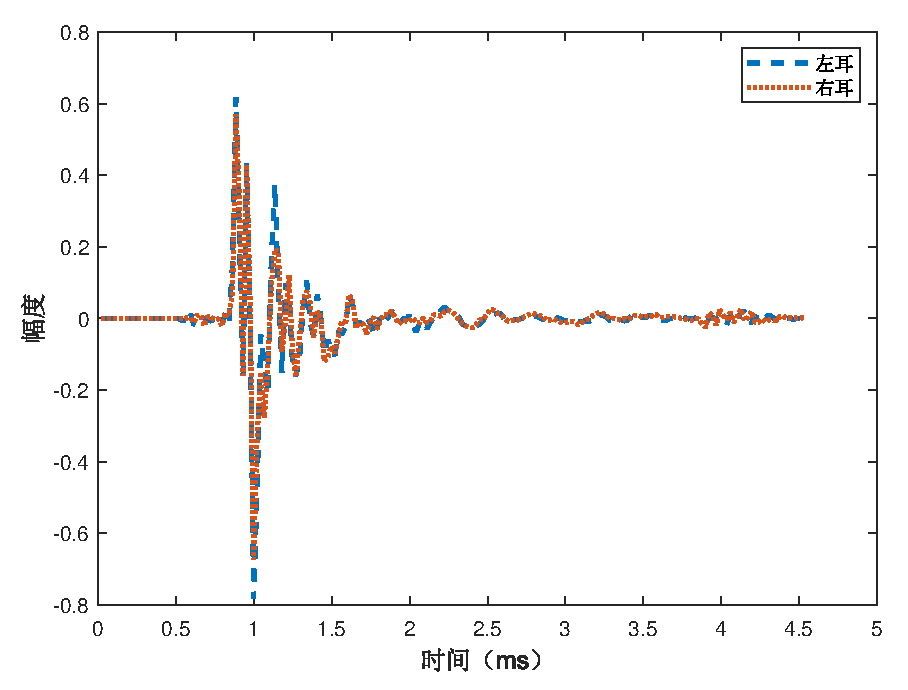
\includegraphics[width=0.48\textwidth]{figure/chapter3/0du_HRIR}}
\hfill
\subfigure[]{
\includegraphics[width=0.48\textwidth]{figure/chapter3/0du_HRTF}}
\caption{CIPIC~数据库中声源位于水平面且方向为~$0^{\circ}$~时的左右耳~HRIR~和~HRTF~数据:(a)~HRIR,(b)~HRTF}
\label{fig:CIPIC_0du}
\end{figure}

% 由于测量系统的力学和物理特性,所测量的HRTFs将不可避免地包含一定的噪声。为了避免噪声的影响,此处的结果展示采用~MESH2HRTF~数据库。


\subsection{HRTF~的球谐系数估计}\label{subsec.HRTF_coe}

% 突然想到一个问题,对于HRTF的分解求解,之前用的是空心球的公式,但是人头是不是应该用刚球? 但人头好像又不能看作是刚性球,刚性球是有条件的,人头的散射反射又不能忽略。  因此不能看作是刚球,所以还是应该使用空心球的公式进行计算。

由于~CIPIC~数据库采用双耳极坐标系,与球谐函数的角度定义不一致,所以在~HRTF~球谐分解之前,需要对~CIPIC~数据库的角度进行转换。
在转换过程中也可以借助~CIPIC~数据库的~SOFA~格式数据,在~SOFA~格式中,角度定义与图~\ref{fig:harmonics_theta_phi_definition}~类似,仅在俯仰角~$\theta$~的定义上不同,其俯仰角为方向矢量与水平面的夹角。

同时为了方便分析,本文对方位角重新定义。 图~\ref{fig:harmonics_theta_phi_definition}~中的俯仰角~$\theta$~为方向矢量与~$z$~正轴的夹角,$\theta=0^{\circ}~,~90^{\circ}~,180^{\circ}~$~分别表示正上方、水平面和正上方,其中水平面是指由原点指向正前方和正右(或左)方的两矢量决定的平面。方位角~$\phi$~为方向矢量在水平面的投影与中垂面的夹角,在水平面上,$\phi=0^ {\circ}~,~90^{\circ}~,180^{\circ}~,270^{\circ}~$~分别表示正前、正左、正后和正右方。
调整后,俯仰角不变,在水平面上,方位角~$\phi=0^{\circ}~,~90^{\circ}~,180^{\circ}~,270^{\circ}~$~分别表示正前、正右、正后和正左方。详见表格~\ref{tab.angel_transform}。

\begin{table}[H]
\centering
\caption{转换前后的角度定义}
\begin{tabular}{|c|c|c|c|}
\hline
   & SOFA~格式角度定义 & 球谐函数角度定义 & 最终角度定义 \\
\hline
俯仰角~$\theta$ & 矢量与水平面的夹角 &  矢量与~$x$~正轴的夹角& 矢量与~$x$~正轴的夹角  \\
 & $-90^{\circ} \leq \theta \leq 90^{\circ} $ & $0 \leq \theta \leq 180^{\circ} $ & $0 \leq \theta \leq 180^{\circ} $ \\
\hline
正上方 & $\theta = 90^{\circ}$ & $\theta = 0^{\circ}$ & $\theta = 0^{\circ}$ \\
水平面 & $\theta = 0^{\circ}$ & $\theta = 90^{\circ}$ & $\theta = 90^{\circ}$ \\
正下方 & $\theta = -90^{\circ}$ & $\theta = 180^{\circ}$ & $\theta = 180^{\circ}$ \\
\hline
正前方 & $\phi = 0^{\circ}$ & $\phi = 0^{\circ}$ & $\phi = 0^{\circ}$ \\
正右方 & $\phi = 270^{\circ}$ & $\phi = 270^{\circ}$ & $\phi = 90^{\circ}$ \\
正后方 & $\phi = 180^{\circ}$ & $\phi = 180^{\circ}$ & $\phi = 180^{\circ}$ \\
正左方 & $\phi = 90^{\circ}$ & $\phi = 90^{\circ}$ & $\phi = 270^{\circ}$ \\
\hline
\end{tabular}
\label{tab.angel_transform}
\end{table}

从~SOFA~格式角度定义到最终角度定义的转换公式为:
\begin{align}
\phi & = mod~\left( 360^{\circ}-\phi_{\text{SOFA}}, 360^{\circ} \right) \nonumber \\
\theta & =  90^{\circ} - \theta_{\text{SOFA}},
\end{align}
其中,$mod$~表示取余。

接下来对进行角度转换后的~HRTF~数据进行球谐分解。由~\ref{sec.SHdecomposition}~节可知,$P$~个方位的~HRTF~可以使用球谐函数进行分解:
\begin{equation}\label{HRTF_decomposition}
H_{\text{L,R}}(\theta_{p},\phi_{p},f)  = \sum_{n=0}^{N_{h}}\sum_{m=-n}^{n} \beta_{nm}^{L,R}(f)Y_{n}^{m}(\theta_{p},\phi_{p})
\end{equation}

球谐系数的求解方式~$\beta_{nm}^{L,R}(f)$~的方法与式~\eqref{eq.coeMat_random_sampling}~类似:
\begin{equation}
\bm{H}_{\text{L,R}} = \bm{Y} \bm{\beta_{nm}}^{\text{L,R}},
\end{equation}
其中,$\bm{Y}$~是大小为~$P \times (N_{h}+1)^2$~的矩阵,$\bm{H}_{\text{L,R}}$~和~$\bm{\beta_{nm}}^{\text{L,R}}$~是长度为~$P$~和~$(N_{h}+1)^2$~的列向量,
\begin{equation}
\bm{Y}=\left[
\begin{array}{ccccc}
Y_{0}^{0}\left(\theta_{1}, \phi_{1}\right) & \cdots & Y_{n}^{m}\left(\theta_{1}, \phi_{1}\right) & \cdots & Y_{N_{h}}^{N_{h}}\left(\theta_{1}, \phi_{1}\right) \\
Y_{0}^{0}\left(\theta_{2}, \phi_{2}\right) & \cdots & Y_{n}^{m}\left(\theta_{2}, \phi_{2}\right) & \cdots & Y_{N_{h}}^{N_{h}}\left(\theta_{2}, \phi_{2}\right) \\
\vdots & \ddots & \vdots & \vdots  & \vdots \\
Y_{0}^{0}\left(\theta_{P}, \phi_{P}\right) & \cdots & Y_{n}^{m}\left(\theta_{P}, \phi_{P}\right) & \cdots & Y_{N_{h}}^{N_{h}}\left(\theta_{P}, \phi_{P}\right)
\end{array}\right],
\end{equation}
\begin{equation}
\bm{H}_{\text{L,R}} = [H_{\text{L,R}}(\theta_{1},\phi_{1},f),~H_{\text{L,R}}(\theta_{2},\phi_{2},f)~,~\cdots~,~H_{\text{L,R}}(\theta_{P},\phi_{P},f)]^{T},
\end{equation}
\begin{equation}
\bm{\beta_{nm}}^{\text{L,R}} = [\beta_{0,0}^{\text{L,R}}~,\cdots,~\beta_{n,m}^{\text{L,R}}~,~\cdots~,~\beta_{N_{h},N_{h}}^{\text{L,R}}]^{T}.
\end{equation}


对于~HRTF~数据库来说,球面采样一般较为密集,假设采样点总数满足~$P>(N_{h}+1)^2$~,因此可以采用式~\eqref{eq.HRTF_Pinv}~进行球谐分量的求解。
\begin{equation}\label{eq.HRTF_Pinv}
\bm{\beta_{nm}}^{\text{L,R}} = \bm{Y}^{\dagger}\bm{H_{\text{L,R}}}= (\bm{Y}^{H}\bm{Y})^{-1}\bm{Y}^{H}\bm{H_{\text{L,R}}}.
\end{equation}

球谐分量~$\bm{\beta_{nm}}^{\text{L,R}}$~也可以用于重建任意方位的~HRTF~,又称为~HRTF~插值。任意方向~$(\theta,\phi)$~的~HRTF~的表达式为:
\begin{equation}
\hat{H}_{\text{L,R}}(\theta,\phi,f) = \bm{y} \bm{\beta_{nm}}^{\text{L,R}}.
\end{equation}

其中,$\bm{y} = \left[ Y_{0}^{0}(\theta,\phi)~,~ \cdots~,~Y_{n}^{m}(\theta,\phi)~,~\cdots~,~ Y_{N_{h}}^{N_{h}}(\theta,\phi)\right]$~为重建方位~ $(\theta,\phi)$~对应的球谐函数向量。

\section{HRTF~预处理}\label{sec.HRTF_pre}

从~\ref{sec.SHdecomposition}~节可知,直接使用低阶截断的~HRTF~分量进行双耳渲染会带来许多问题,因此需要引入~HRTF~预处理方法进行改进。一些~HRTF~预处理方法通过寻找对~HRTF~更为紧凑的表示,使大部分能量集中在球谐分解的低阶分量上。本节将对~HRTF~的预处理方法之一~——~双耳对准加以介绍,并且通过实验验证了该方法的有效性。




\subsection{预处理方法}

为了降低~HRTF~的低阶球谐表示所引起的误差,建议引入预处理来降低~HRTF~的有效球谐阶数。
对于式~\eqref{HRTF_decomposition}~中对~HRTF~的球谐分解,其高阶球谐分量主要是由高频处快速的相位变化导致的。并且研究表明,去除或者改变高频处的双耳相位差~(interaural phase difference~,~IPD)~在感知上无关紧要~\tcite{2015Efficient}。在此基础上,对~HRTF~进行相位修正的预处理方法被用于~HRTF~低阶球谐分解的扩展工作。
例如,对高频应用时间对准,即通过减去高频部分的线性相位部分来实现~IPD~均衡~\tcite{2018Binaural}\tcite{2018comparison},可以降低~HRTF~数据库的空间复杂度,从而降低所需的球谐分解阶次。


知觉研究表明,听觉系统在判断声源方位时所使用的声学信息是有选择性的,在自由场情况下,人耳听觉系统对单一声源进行定位时,主要定位因素双耳时间差~ITD~和双耳声级差~ILD~随着频率的作用范围如下所示:
\begin{compactitem}
\item 在频率小于~1.5~kHz~的情况下,双耳时间差~ITD~是方向定位的主要因素;
\item 在频率为~1.5~kHz~到~4~kHz~的情况下,双耳时间差~ITD~和双耳声级差~ILD~对方向定位共同起作用;
\item 在频率大于~4~kHz~到~5~kHz~的情况下,双耳声级差~ILD~是方向定位的主要因素。
\end{compactitem}


基于高频处~HRTF~的幅度部分对定位的感知起决定作用这一事实,在本研究中,采用了与之前相同的处理方法,对高频相位加以修正。主要关注对高频处~HRTF~幅度的近似,而相位从临界频率开始加以改变。

加以相位对准的头相关传递函数~
$H_{\text{L,R}}^{a}(\theta,\phi,f)$~可表示为:
\begin{equation}\label{eq.HRTF_pre}
H_{\text{L,R}}^{a}(\theta,\phi,f) =
\begin{cases}
 H_{\text{L,R}}(\theta,\phi,f)  ,  & f<f_{c} \\
 H_{\text{L,R}}(\theta,\phi,f) e^{i\zeta} , & f \geq f_{c},
\end{cases}
\end{equation}
其中,$f_{c}$~为临界频率,一般选取~1.5~kHz。对于给定的频率,$\zeta$~的表达式为:
\begin{align}
\zeta & = \angle \left(~ [ H_{\text{L,R}}(\theta,\phi,f)]^{*} H_{\text{L,R}}(\theta,\phi,f_{c})~\right) \nonumber \\
& = \angle \left(~ H_{\text{L,R}}(\theta,\phi,f_{c}) ~\right) - \angle \left(~ H_{\text{L,R}}(\theta,\phi,f) ~\right),
\end{align}
其中,$\angle(\cdot)$~表示取一个复数的相位信息。

上述公式给出了直接从~HRTF~数据中获取相位差的方法,也可以根据声源方位和人头尺寸等参数获取,如下所示:
\begin{equation}\label{eq.time_align}
\zeta = 2\pi (f_{c} - f) \tau_{p}^{\text{L,R}},
\end{equation}
其中,$\tau_{p}^{\text{L,R}}$~为声源位于~$(\theta_{p},\phi_{p})$~位置处对应的时间偏移,即头中心和耳朵之间的时间差。

假设为远场条件,此时声源信号可以看作平面波,因此$\tau_{p}^{\text{L,R}}$~的计算公式为:
\begin{equation}
\tau_{p}^{r}=\cos \left(\theta_{p}\right) \sin \left(\phi_{p}\right) a/c, \quad \tau_{p}^{l}=-\tau_{p}^{r}
\end{equation}

使用式~\eqref{eq.time_align}~通过时间差计算相位差从而对~HRTF~进行对准的方法一般被称为时间对准。时间对准的~HRTF~和相位对准的~HRTF~方法的原理基本一致,核心思想是将原有的~HRTF~中使用自由场下头中心处的声压对双耳声压进行归一化转换为使用双耳所在位置的声压对双耳声压进行归一化,此处方法已被证明是一种有效降低~HRTF~SH~阶次的稳健方法,有很多工作基于此进行~\tcite{2018Binaural}\tcite{2019Efficient}\tcite{ben2020binaural}。

和直接使用最小二乘方法求解头相关传递函数的球谐分量相比,该预处理方法一方面准确地表示头相关传递函数的幅度谱,并有效降低了头相关传递函数的分解阶次。

请注意,与其他以前建议的有效的~HRTF~表示方法不同,该相位校正过程是可逆的,这意味着从原始~HRTF~到经过对准的~HRTF~再到原始~HRTF~不会丢失任何信息。

\newpage
\subsection{实验结果与分析}\label{sec.Pre_result}

为了衡量~HRTF~预处理算法对球谐分解所带来的影响,定义~HRTF~球谐分解分量在~$n$~阶下的能量~$E_{\text{L,R}}(f,n)$~和所有阶次下的累积能量~$E_{\text{L,R}}^{C}(f,n)$~为:
\begin{equation}
E_{\text{L,R}}(f,n) = \sum_{m=-n}^{n} | \beta_{nm}^{\text{L,R}}(f) |^{2},
\end{equation}
\begin{equation}
E_{\text{L,R}}^{C}(f,n) = \sum_{n=0}^{N_{h}} \sum_{m=-n}^{n} | \beta_{nm}^{\text{L,R}}(f) |^{2}.
\end{equation}

为了避免测试环境对预处理前后阶次变化的影响,本节采用消声室环境下使用~Neumann~KU-100~在~2702~点球面列别捷夫采样下的远场数据库~\tcite{Benjamin2013A}。在计算过程中,对能量进行归一化,并对归一化能量取对数~$10\text{lg}\left( E_{\text{L,R}}(f,n)\right)$。预处理前后的球谐分量的能量分布如图~\ref{fig:pre_after}~所示,图中黑色实线表示有效球谐分解阶次,即前~$N$~阶球谐分量包含了~HRTF~$99\%$~的能量。

\begin{figure}[H]
\centering
\subfigure[]{
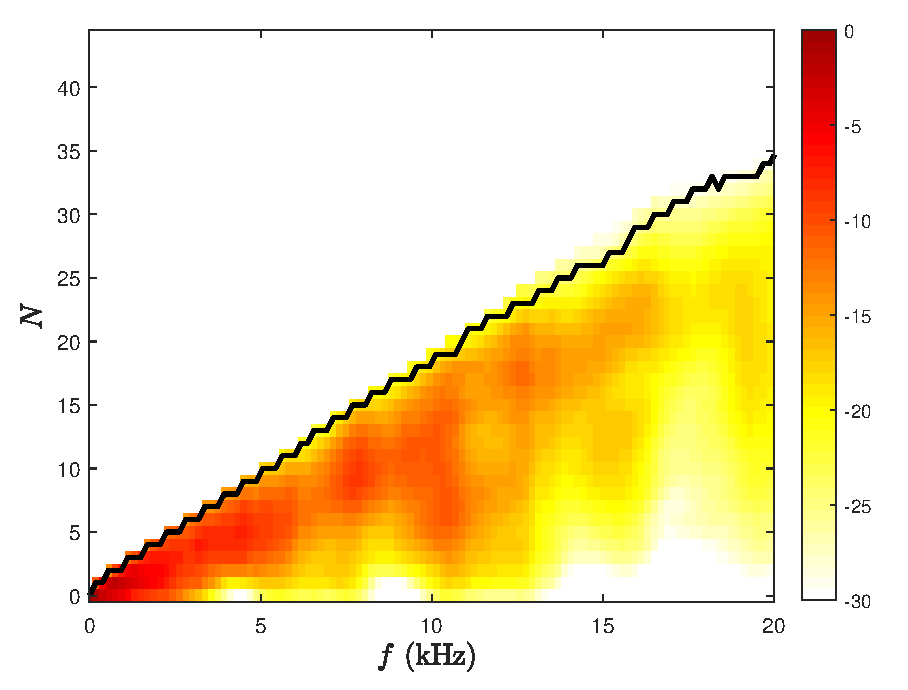
\includegraphics[width=0.48\textwidth]{figure/chapter3/nopre}}
\hfill
\subfigure[]{
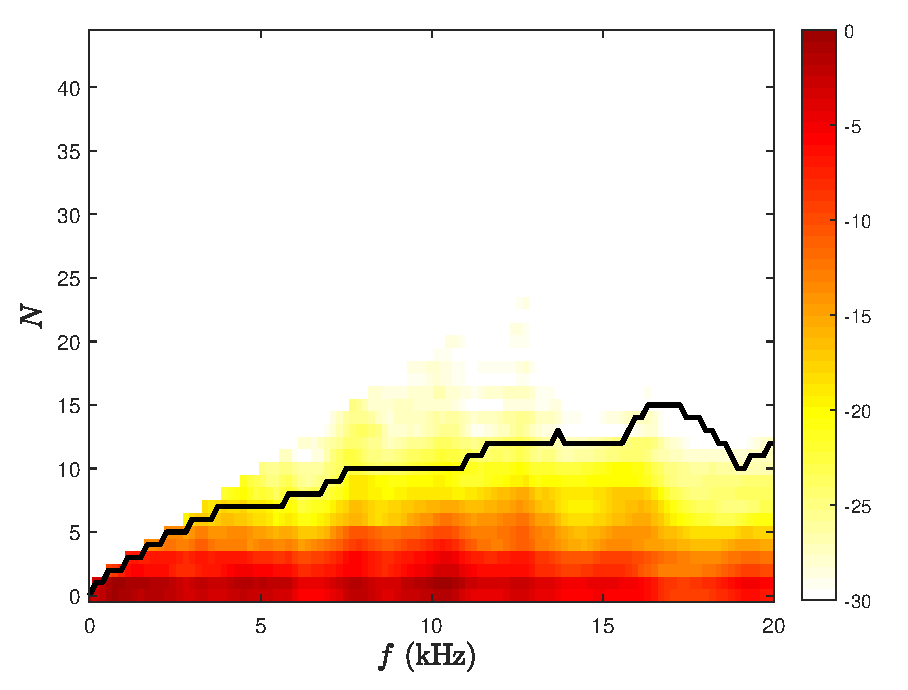
\includegraphics[width=0.48\textwidth]{figure/chapter3/pre}}
\caption{预处理前后~HRTF~的能量分布:~(a)预处理前,(b)预处理后}
\label{fig:pre_after}
\end{figure}


从图~\ref{fig:pre_after}~可以看出:
\begin{inparaenum}[(1)]

\item 未引入预处理时,HRTF~球谐分解所需阶次较大,并且随着频率的增加,球谐分解阶次逐渐增加;

\item 对头相关传递函数加以预处理后,HRTF~球谐分解所需阶次较小,并且随着频率的增加,球谐分解阶次趋于稳定;

\item 与频率相关的双耳对准预处理算法可以有效降低~HRTF~的分解阶次,由原来的~34~阶降低至~15~阶。

\end{inparaenum}

\section{本章小结}

本章对基于球谐分解的双耳渲染进行了详细的理论推导,并针对其存在的不匹配问题,对~HRTF~进行预处理。 首先,对声场的球谐系数估计进行推导,并且针对空心球和刚性球两种情况给出了不同的计算方法。其次对~HRTF~数据库、HRTF~的球谐系数估计以及对~HRTF~数据库进行球谐分解的前提~——~角度转换进行了详细介绍。并引入~HRTF~预处理方法,以降低~HRTF~的球谐分解阶次和提升双耳感知。实验结果表明,与频率相关的双耳对准预处理算法可以有效降低~HRTF~的分解阶次。

